\section{Compilation}
\label{sec:compilation}


\subsection{Overview}

\begin{figure}[t!]
\centering
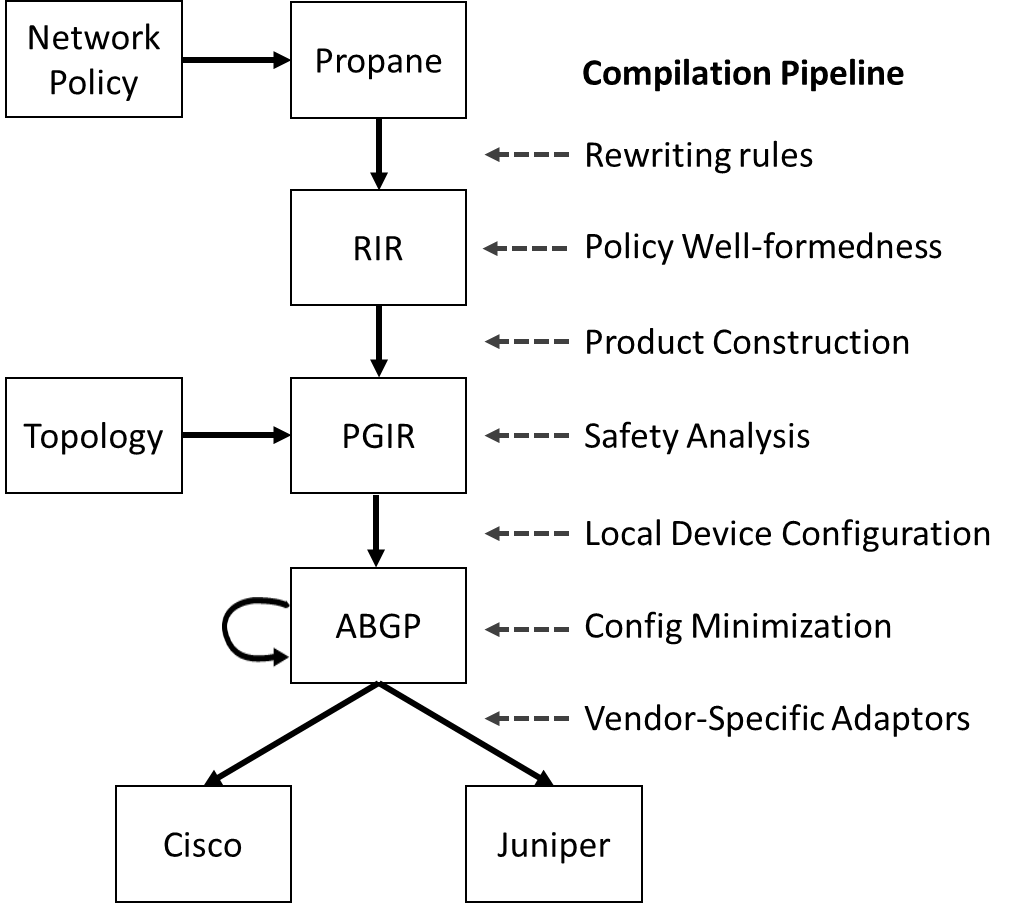
\includegraphics[width=\columnwidth]{figures/pipeline}
\caption{Compilation pipeline stages for Propane.}
\label{fig:pipeline}
\end{figure}

In this section we briefly describe our compilation strategy for \sysname. Figure~\ref{fig:pipeline} shows the 5 stage compilation pipeline to translate user-level \sysname policies into vendor-specific, device-local BGP policies. The first stage of the pipeline involves simple rewriting rules and substitutions from the user-level languae into the core Regular Intermediate Representation (RIR). Policies in RIR are checked for well-formedness (e.g., never constraining traffic that does not enter the network), before being combined with topological information to obtain Product Graph Intermediate Representation (PGIR). The PGIR is a data representation that compactly captures the control flow of all BGP advertisements subject to the policy and topology restrictions. We develop efficient algorithms that operate over the PGIR to ensure policy compliance, guarantee failure safety, avoid BGP instability, and prevent aggregation-induced black holes. Once the compiler determines the PGIR for the policy is safe, the compiler uses a simple translation to an abstract BGP (ABGP) representation. To make configurations more readable for human operators, and to reduce the size of the resulting configurations, the \sysname compiler makes several passes over ABGP form. Finally, vendor-specific adaptors can be added to \sysname to translate from ABGP to actual concrete configurations that go on the network devices.


\subsection{Regular IR (RIR)} 
\label{sec:rir}

The high-level language presented in Section~\ref{sec:propane} is just a thin layer on top of a core, regular-expression-based language for describing preference-based path constraints. Regular expressions are an expressive formalism that have been studied extensively for their ability usefulness in describing paths through graphs~\cite{bib:todo}. We prese

\para{Syntax}
Define the grammar of each of the languages - regular language, the macro language on top of it, and maybe the IR language.

% grammar
\newcommand{\BNFALT}{\;\;|\;\;}
\newcommand{\hdr}[2]{\flushleft \chdr{#1}{#2}}
\newcommand{\chdr}[2]{\textbf{#1} {#2} \\ \centering}

\begin{figure*}
  \begin{minipage}[t]{.45\linewidth}
  \hdr{\large Syntax}{}
  \vspace*{-1\baselineskip}
  %
  \[ \begin{array}{rclr}
    \hline

     pol     &::=& p_1, \dots, p_n & \textit{constraints} \\
     p       &::=& t \mapsto r_1 \gg \dots \gg r_m & \textit{preferences} \\
     t       &::=& & \textit{test} \\
         &\BNFALT& true & \textit{true} \\
         &\BNFALT& \neg t & \textit{negation} \\
         &\BNFALT& t_1 \vee t_2 & \textit{disjunction} \\
         &\BNFALT& t_1 \wedge t_2 & \textit{conjunction} \\
         &\BNFALT& prefix = x & \textit{prefix test} \\
         &\BNFALT& comm = c & \textit{community test} \\
     r       &::=& & \textit{regular paths} \\ 
         &\BNFALT& n & \textit{AS number} \\
         &\BNFALT& in & \textit{internal loc} \\
         &\BNFALT& out & \textit{external loc} \\
         &\BNFALT& r_1 \cup r_2 & \textit{union} \\
         &\BNFALT& r_1 \cap r_2 & \textit{intersection} \\
         &\BNFALT& r_1 \cdot r_2 & \textit{concatenation} \\
         &\BNFALT& !(r) & \textit{path negation} \\
         &\BNFALT& r^* & \textit{repetition} \\
     l       &::=& r_1 \rightarrow r_2 & \textit{link pairs} \\
     cc     &::=& agg(x, l) \BNFALT tag(c, t, l) & \textit{control constraints} \\
  \end{array} \]

  \end{minipage}
  %
  ~~
  \vrule
  ~~
  %
  \begin{minipage}[t]{.5\linewidth}
  \hdr{\large Propane Expansions}{}
  \vspace*{-1\baselineskip}
  %
  \[ \begin{array}{rcl}
    \hline
    any           & = & out^* \cdot in^+ \cdot out^* \\
    internal      & = & in^+ \\
    external      & = & out^+ \\
    only(X)       & = & any \cap X^* \\
    never(X)      & = & any \cap (!X)^* \\
    through(X)    & = & out^* \cdot in^* \cdot X \cdot in^* \cdot out^* \\
    after(X)      & = & out^* \cdot (X \cap out) \cdot out^* \cdot in^+ \cdot out^* \\
    before(X)     & = & out^* \cdot in^+ \cdot out^* \cdot (X \cap out) \cdot out^* \\
    end(X)        & = & any \cap (\Sigma^* \cdot X) \\
    start(X)      & = & any \cap (X \cdot \Sigma^*) \\
    exit(X)       & = & (out^* \cdot in^* \cdot (X \cap in) \cdot out \cdot out^*) \cup \\
                  &        & (out^* \cdot in^+ \cdot (X \cap out) \cdot out^*) \\
    enter(X)      & = & (out^* \cdot out \cdot (X \cap in) \cdot in^* \cdot out^*) \cup \\
                  &        & (out^* \cdot (X \cap out) \cdot in^+ \cdot out^*) \\
    link(X,Y)     & = & any \cap (\Sigma^* \cdot X \cdot Y \cdot \Sigma^*) \\
    path(\vec{X}) & = & any \cap (\Sigma^* \cdot X_1 \dots X_n \cdot \Sigma^*) \\
    novalley(\vec{X}) & = & any ~ \cap \\
                  &   & !path(X_2,X_1,X_2) ~ \cap \dots \cap \\ 
                  &   & !path(X_n,X_{n-1},X_n) \\
  \end{array} \]

  \end{minipage}

  \hrulefill

  \caption{Regular Intemediate Language (RIL) syntax (left), and 
           Propane language expansions (right).}
  \label{fig:semantics}
\end{figure*}

\para{Semantics}
Give the semantics in terms of ranked paths.
Extension of regular expression semantics with the
additional constraint that we take only valid topology paths and that their are no paths with
repeated locations in the path. One tricky point is that we care about paths starting or ending at locations that are
connected to end-hosts in some way. And we want the length of the path to be a secondary tie-breaker.

\para{Propane to RIR}

TODO



\subsection{Theory}
What are the properties of this language? Ideally, a proof here about its expressiveness. We can perhaps do everything
BGP can do? We can't do shortest paths routing with BGP, but we could with OSPF though? Clearly we can only describe
policies that are stable under all possible failure scenarios (at least internally stable, could still cause) routing
loops with interactions with neighbors.











\begin{itemize}
	\item Separate prefixes so they are disjoint
	
	\item For each prefix, build a DFA from each of the regular path constraints
		  We do this using character classes and regular expression derivatives.
		  The accepting states are labeled with the particular preference.
	
	\item Build the constraint graph, which gives us valid paths through the network that satisfy one or
		  more of the regular path constraints. We accept if we are in at least one of the accepting states
		  for one or more of the DFAs. Add a new start and end node as well.
		
	\item Minimize the constraint graph by removing nodes and edges that never contribute to a solution.
		  Required for soundness. Removing these makes it easier to check if things are implementable using BGP (see next point).
		  We use several heuristics to make this faster (e.g., removing edges for dominated nodes)
		
	\item Since our policy language can express things not implementable in BGP, we need a few checks.
		  First show some examples of what the problem is: why BGP cannot make a decision.
		  The reasons this can happen are:
		  (1) Single best path per router - no subset of paths specified is consistent (if A goes through B and C goes through A, then C goes through B).
		  (2) Failures - Have to make a decision without knowing what failures have occurred. Never want to prefer one peer over another and then not get a path when one was available

	\item We can check for these with a sufficient condition (that works often and is very fast),

	\item For each router, build a preference pre-order, that defines the constraints between preferences.
	
	\item Finally, if we know BGP can make decision locally, then we can directly translate to local BGP configurations using
		  information about the state machines from the neighbors. In particular, we tag (and test on) community values for the
		  corresponding state and set preferences accordingly (example will be needed)

	\item Running example will be helpful here.	
\end{itemize}


\subsection{Optimizations}

\begin{itemize}
	\item For performance, the main bottleneck will probably be the minimization step. We use a number of heuristics here to make this faster.
	\item For config readability and number of route maps/communities, we avoid community tagging/matching whenever possible with a number of tricks.
\end{itemize}



